\section{Learning a Belief Representation}

In this section, we present our approach to learning a belief representation for constant delays. 
Once learnt, this representation can be used alongside any \gls{rl} algorithm as a substitute for the state.
This approach is then extended to learning more delays simultaneously via a simple ``trick''. 

\subsection{Belief Representation Network}
\label{subsec:belief_net}

To learn the belief $\augmentedbelief(\cdot\vert x)$ for some augmented state $x=(s,a_1,\dots,a_{\delay})\in\augmentedstate$, one should anticipate the effect of the actions contained in the augmented state.
One approach is to approximate the transition dynamics with a recurrent function.
Recurrent \gls{nn} could be considered an approximator, but these networks are slow to train and evaluate.
Instead, we process the entire input directly with a \gls{nn} $f_{\vectorialform{\phi}}$ with parameters $\vectorialform{\phi}$ and ask the network to output the belief representations for all the unobserved states at once.
The network could process the augmented state in many ways.
We choose to form a sequence $(s,a_{i})_{i \in [\![1,\delay]\!]}$ from the augmented state.
This sequence is then fed to the encoder network of a causal Transformer~\cite{vaswani2017attention} (see~\Cref{subsubsec:transformer}) which we refer to as $f_{\vectorialform{\phi}}$. 
The choice of a causal Transformer has been made for mainly threes reasons; the Transformers have achieved great empirical results on sequence-to-sequence tasks \cite{devlin2018bert}; it can be used with a mask to preserve causality, this is useful since past beliefs do not depend on future beliefs; the positional encoding inside the Transformer allows one to add information on the position of the action in the sequence, the same action can therefore have different effects in different positions inside the augmented state. 

To train $f_{\vectorialform{\phi}}$ to effectively encode a belief, we use a \gls{maf}~\cite{papamakarios2017masked} network (see~\Cref{subsubsec:maf}) .
The choice has been based on its ability to approximate probability distributions.
This network, which we note $f_{\vectorialform{\theta}}$, will take the output of $f_{\vectorialform{\phi}}$ as a conditional on its probability. 
Then, it will be trained to approximate the probability of unobserved states only from the condition given by $f_{\vectorialform{\phi}}$. 
In this way, all information about the belief will be encoded in $f_{\vectorialform{\phi}}$.
Note that the loss gradient of a \gls{maf} network can flow through its conditional and therefore can be used to train $f_{\vectorialform{\phi}}$ at the same time.

Let us now delve more precisely into what happens inside the belief network.
Let $x=(s,a_1,\dots,a_{\delay})$ be the current augmented state. First, the Transformer outputs a vector $f_{\vectorialform{\phi}}(x)_i\in\realnumbers^{n_b}$ for each element $(s,a_{i})$ of $(s,a_{i})_{i \in [\![1,\delay]\!]}$. 
We note $n_b$ as the dimension of this representation of the belief. 
Let $(s_1,\dots,s_{\delay})$ be the $\delay$ unobserved states for which the belief will be approximated and $\augmentedbelief[i](\cdot\vert x)$ the belief of $s_i$. 
As explained in \Cref{subsubsec:maf}, \gls{maf} recursively applies parameterized functions to a base density $p_u$ to transform it into the density $p_{\theta}$.  
For the base density $p_u$, we use the normal distribution.
The difference from the traditional setting is that here, compared to \Cref{eq:p_inverted_maf}, we add a conditioning on $f_{\vectorialform{\phi}}({x})_i$.
\begin{align*}
    p_{\vectorialform{\theta}}(s_i\vert f_{\vectorialform{\phi}}({x})_i) = p_u(f_\theta^{-1}(s_i,f_{\vectorialform{\phi}}({x})_i)) \left\lvert \det\left(\frac{\partial f_\theta^{-1}}{\partial s_i}\right)\right\rvert.
\end{align*}
Note that the building block of MAF, the MADE layer (see~\Cref{subsubsec:maf}), requires a single pass to compute a density, while it requires as many passes as the dimension of the output for sampling. 
This is not limiting here, as we are not interested in sampling states from the belief but only learning an approximation of it. 

Then, \gls{maf} is trained to minimise the Kullback-Leibler divergence between its density and the density of the training set. 
Here, the loss reads,
\begin{align*}
    \min_{\vectorialform{\theta},\vectorialform{\phi}} \sum_{i=1}^\delay \kullbackleiblerdivergence( \augmentedbelief[i](s_i \vert  x) \Vert p_{\vectorialform{\theta}}(s_i\vert f_{\vectorialform{\phi}}({x})_i)).
\end{align*}
This quantity is differentiable by design and can be minimised by gradient-based optimisation.
For a sample of $N$ augmented states $(x^k)_{1\le k\le N}$ where $x^k=(s^k,a^k_1,\dots,a^k_{\delay})$, the loss can be approximated as,
\begin{align}
\label{eq:loss_maf}
    \mathcal{L}_p = \sum_{k=1}^N \sum_{i=1}^\delay \log p_{\vectorialform{\theta}}(s^{k}_{i}\vert f_{\vectorialform{\phi}}(x^k)_i). 
\end{align}
A graphical representation of the belief representation network is given in \Cref{fig:dtrpo_network} and its training is described in \Cref{algo:belief_training}.
It is common to use a replay buffer in \gls{rl} to compensate for a sampling policy that evolves over time due to training.
This also brings the framework closer to supervised learning. 
We use the same idea here by saving the augmented states in a replay buffer. 

The belief representation network can be used along any \gls{rl} algorithm as a pre-processing of the state. 
In the experimental section, we plug this network to \gls{trpo} \cite{schulman2015trust} and call the approach Delayed-TRPO (D-TRPO).

\begin{figure}[t]
    \centering
    \resizebox{10cm}{!}{%
    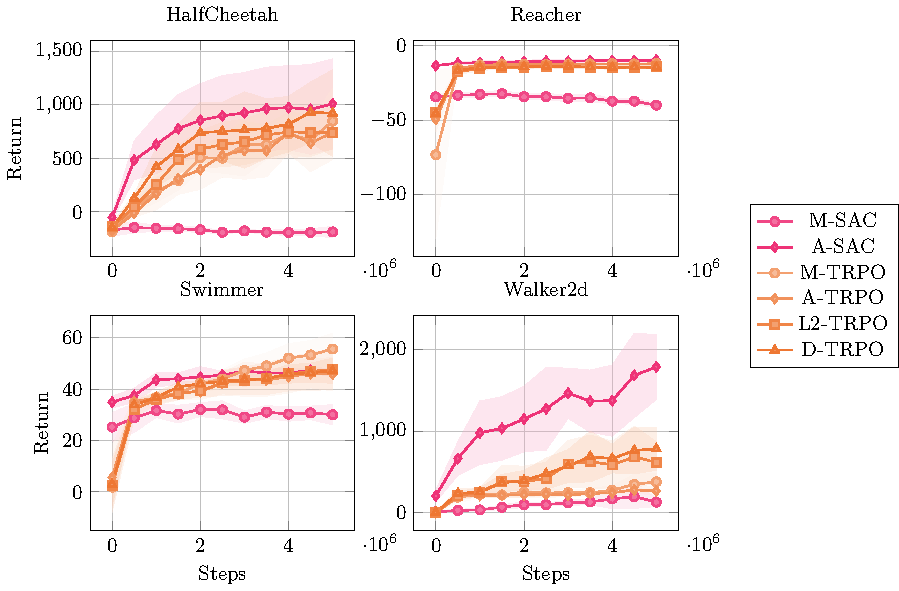
\includegraphics[labelbelief=dtrponetwork]{img/thesis_plots_belief.pdf}
    }
    \caption{The D-TRPO network. From bottom to top; the augmented state is split in a series $(s,a_{i})_{i \in [\![1,\delay]\!]}$; the series is passed through a Transformer encoder layer to return belief encodings $f_{\vectorialform{\phi}}(x)_i\in\realnumbers^{n_b}$; a MAF layer learns the belief of the next $\delay$ states conditioned on the previous encoded vector. Finally, the last belief encoding $f_{\vectorialform{\phi}}(x)_\delay$ is used as input to the policy.}
    \label{fig:dtrpo_network}
\end{figure}


\begin{algorithm}[t] 
\caption{Belief representation network training}\label{algo:belief_training}
\textbf{Inputs}:
belief representation network parameters $\vectorialform{\phi}$ and $\vectorialform{\theta}$, number of epochs $K$, batch size $N$,number of samples $M$, empty replay buffer $\mathcal{D}$.\\
\textbf{Outputs}: Trained parameters $\vectorialform{\phi}$ and $\vectorialform{\theta}$.
\begin{algorithmic}[1]
    \FOR{$k=1,\dots,K$}%\{$1,\dots,N$\}}
        \STATE Collect $M$ samples under some policy $\pi$ 
        \STATE Add couples of augmented states $x=(s,a_1,\dots,a_{\delay})$ and corresponding sequence states to be predicted $(s_1,\dots,s_\delay)$ to $\mathcal{D}$
        \STATE Sample $N$ such couples from $\mathcal{D}$
        \STATE Update parameters $\vectorialform{\phi}$ and $\vectorialform{\theta}$ by descending the gradient $\nabla_{\vectorialform{\phi},\vectorialform{\theta}}\mathcal{L}_p$ (See \Cref{eq:loss_maf})
    \ENDFOR
\end{algorithmic}
\end{algorithm} 

\subsection{Learning Multiple Delays at Once}
\label{subsec:multi_delay_once_belief}
We propose a simple idea to take advantage of the policy learnt by D-TRPO for a given integer delay $\delay>0$.
Despite its simplicity, the previous literature has not considered this idea.
We propose to apply D-TRPO to smaller integer delays $0<\delay'<\delay$ by simulating a delay of $\delay$.
To do so, in addition to the augmented state $x_t=(s_{t-\delay'},a_{t-\delay'},\dots,a_{t-1})$ considered for a delay $\delay'$, we consider a buffer,
\begin{align*}
    (s_{t-\delay},a_{t-\delay},\dots,s_{t-\delay'-1},a_{t-\delay'-1}),
\end{align*} 
of the last $\delay-\delay'$ states and actions in the history before $t-\delay'$.
In this way, the agent can construct a synthetic augmented state $x_t'=(s_{t-\delay},a_{t-\delay},\dots,a_{t-1})$.
This is sufficient to apply the policy learnt by D-TRPO on delay $\delay$. 
Obviously, this algorithm has the same performance guarantee as D-TRPO for delay $\delay$.
We provide experiments in \Cref{sec:exp_belief} to illustrate the effectiveness of the idea. 

For some approaches from the literature, one could do better than the above simple idea.
For example, similarly to \cite{firoiu2018human}, instead of learning a representation of the belief, we could learn the expected future state for all the $\delay$ states to come. 
We design an approach to do so, using the same network structure as for D-TRPO but removing the MAF layer. 
We train the network to minimise the L2 loss between its outputs $(f_\phi(\textbf{x})_i)_{i\in[\![1, d]\!]}$ and the true states $(s_1,\dots,s_\delay)$.
Plugged to \gls{trpo}, we call this approach L2-TRPO.
In this case, we can learn multiple delays at once in another way. 
Indeed, an interesting property of the causal Transformer network is that it can be sliced to the desired length and can therefore be applied to the augmented state of a shorter delay $0<\delay'<\delay$.
By design, L2-TRPO has also learnt the expected state $\delay'$ in the future.
Therefore, the output of the sliced Transformer can be used as input to \gls{trpo}.
Notably, this cannot be done with D-TRPO. Although it learns a representation of the belief for each of the $\delay$ states to come, their respective encoding might follow different rules. 
Therefore, \gls{trpo} may not be able to understand the encoding of a previous state.

The simple idea presented here resonates with the argument of \cite{chen2021delay} that model-based methods are better for delays because their model can be reused.


